\chapter{Implementation}
\label{chap:ch4_abbr}
\label{chap:figtab}
\section{Review}
The software implementation showcase the functionality of all the requirements as described previously. This functionality include the ability to input data and retrieve data through the system. This was accomplished by taking measures provide maximum result as required. This measures include the choice of tools used for the development and the design approach. It was implemented to demonstrate the realization of the proposed specifications especially features such as making reservations in the system.
\section{Implementation tools}
 The user interface is implemented on the internet web browser using local server port as web address. The web browser serves as the environment for testing and implementing the front-end (user interface) of the software, and while the HTML template and Go library is used for the development. The database was developed using the SQLite model schema. The Go HTTP server provides connections between the front-end and back-end implementation. It servers as a channel for parsing request through user interface and database. We used a local TCP network for this implementation.  These tools provided all the necessary component to address the requirements for this software. 
\section{Program Structure}
The Go programming language has a fundamental development structure that is categorized into packages. The packages contains a group of program file with dependencies that links them together. For this software design, we have written two main package to actualize the development goal. These packages includes:
\begin{description}
\item[$\bullet$]Database package 
\item[$\bullet$]HTTP package 
\end{description}

The database package contains all the Go files with database related struct (class). The Go objects represent the same data as in the database. And each Go struct depends on this package as the object-relational mapping tool (ORM) between other struct and database resources. The HTTP package also contain some Go file relates to the user interface ( for example the function Handler) and HTML files. the HTML files contains several templates for the web interface content and elements. These file depends on the HTTP package for serving the web contents and post requests. Below is a table describing the list of files in each packages.
\pagebreak
\begin{table}[h!]
  \centering
  \label{tab:table1}
  \begin{tabular}{ccc}
    \hline
    No & Package & Files\\
   \hline
    1 &Database (pkg)& machine.go\\
       &&reservation.go\\
      &&disk.go\\
      &&user.go\\
      &&nic.go\\
    \hline
    2 &HTTP (pkg)& handler.go\\
    &&server.go\\
    &&Templates(.html)\\
    \hline
  \end{tabular}
  \caption{Program packages}
\end{table}

\section{List of Struct and methods}
Figure \autoref{fig:Description of Methods} shows the class diagram of the list of struct and methods with their relationships with others. It shows the group of methods that perform the tasks specified in the software requirement in our design.
\begin{figure}[h!]
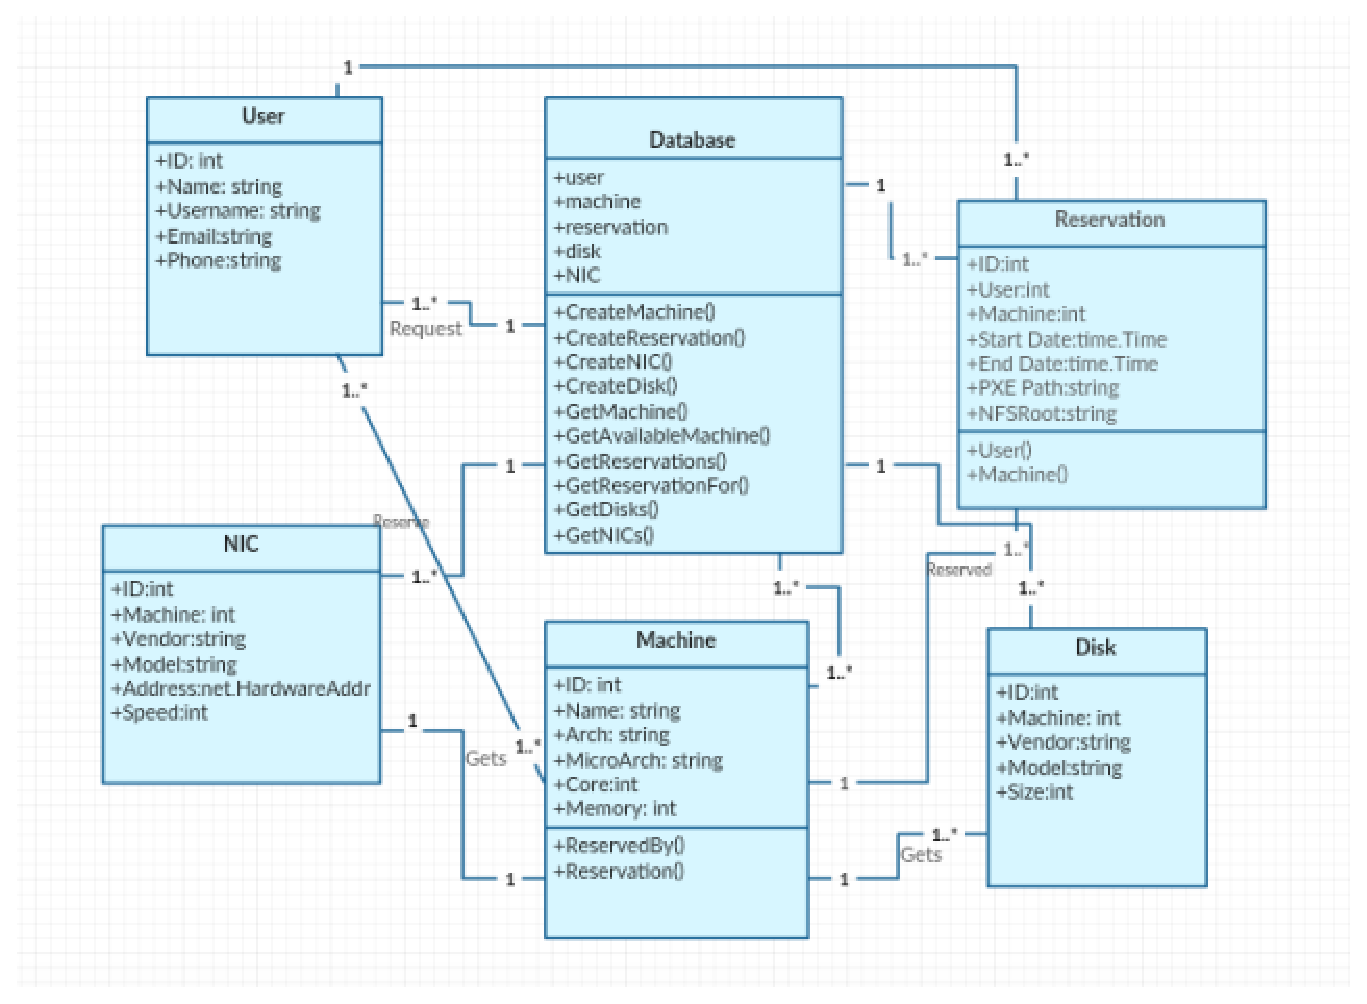
\includegraphics[width = \linewidth]{methods.eps}
\label{fig:Description of Methods} 
\caption{Class Diagram showing struct and method relationships}
\end{figure}
\pagebreak
\section{Description of Methods}
\section*{Adding Machines to the system}
Adding machines and other devices to the system is one of the software requirements in section \ref{addmachines}. On the user interface, the software provides a text field and forms where users can enter details of machines to be saved as data in the database. The InitMachine method create a new database schema with defined table fields where data is stored. When the user submits a Add Machine form, the InitMachine create the database schema where the machine details is stored. It uses type (Machine) fields as argument for creating the schema fields. Below is the code listing for creating database:
\lstset{basicstyle=\footnotesize\ttfamily,breaklines=true}
\lstset{framextopmargin=50pt,frame=bottomline}
\begin{lstlisting}[caption=Creating Database for machine, label=Initializing database]
func initMachines(tx *sql.Tx) error {
	_, err := tx.Exec(`
	CREATE TABLE Machines(
		...........
	);`)
	return err
}
\end{lstlisting}

The CreateMachine method is responsible for parsing the data to the database schema. It uses the SQL INSERT query to parse a give data using the arguments to the database. When the user submit a form (AddMachine), the Go HTTP handler process this form by converting the plan text to a form data according to their data types defined in the schema, and then call the CreateMachine to insert this data to the database. Below is the code list:

PSEUDOCODE:\linebreak
1 Set the table fields .
2 Insert into values into the fields.
3 If value format is valid, stored values and return.

\begin{lstlisting}[caption=Adding machines details, label=Adding machine]
func (d DB) CreateMachine(name string, arch string,
	microarch string, cores int, memoryGB int) error {
	_, err := d.sql.Exec(`
			INSERT INTO Machines(name, arch, microarch,
			 cores, memory)
			VALUES (
				//field values
			)`,
		name, arch, microarch, cores, memoryGB)
	return err
}
\end{lstlisting}

\section*{Making a Reservation}
The reservation process is similar to creating a machine but here it requires the User ID and Machine ID as foreign keys in creating the database schema. The User ID is used for selecting the user making the reservation, and Machine ID for selecting the machine to be reserved. On the web interface (reservation page), the form has a drop down list where users can select their user name and the machine they want to reserve. When users open the reservation page to create new reservation, the HTML form use the post request to get list of machines and user name on the drop-down list.
PSEUDOCODE:\linebreak
1 Input reservation values in the field.
2 Select machine id from the list where machine name is chosen.
3 Select user id from the list of user where name is chosen.
4 Insert all the values to reservation table and return.
\begin{lstlisting}[caption=Storing Reservation details, label=Adding reservation]
	_, err := d.sql.Exec(`
			INSERT INTO Reservations(machine,user,start,end,
			pxepath,nfsroot)
			VALUES (
				(SELECT id from Machines where name=?),
				(SELECT id from Users where username=?),
				//other fields
			)`,
\end{lstlisting}

To make a reservation, users will select their user name and a machine from the drop down list which is loaded by GetMachine and GetUser method. The selection query gets the User ID and the Machine ID of the selected user name and machine as foreign key to the reservation database schema. Also, start and end time/date of the reservation is entered on the text field , and this plain text is formatted to match the database using a time package in Go library. After submitting the form, the Go HTTP handler handles the Insert query by taking all the argument values and saving them to database. 
\section*{Checking Available Machines}
The user can search the inventory for specific imformation. One of the example is the ability to search for available machines in the system as one of the requirement \ref{searchinventory}. Available machines are those machines that are free for a certain period. This feature helps users to get list of machine free to be reserved. In this process of checking available machine, the user enters a specific start date and end date in the provided text feild, and submits the query. After submiting the query, the HTTP handler processes this request, and the server calls the GetAvailableMachine method to fetch this request from the database. Go HTTP handler uses a Request functon to call the server and  ResponseWriter to respond to the HTML request \cite{Gohttp}. The server uses ListenAndServe method to listen to incoming request and to call the requested method to handle the request. In this method, we used a SQLite JOIN sub query to combine the machine and reservation database table. This combination logic allows the query to scan through both table rows using reservationID and machineID to indentify the machines that are not reserved for that time range the user entered. The logic contains SQL WHERE, OR and AND operator to perform comparisons between reservation dates and time. \cite{ANDOR}The AND operator is used to allow multiple conditions in the statement,  the OR operator is used to combine condition that are true, and the WHERE clause is used to specify condition while fetching data from database\cite{WHEREclause}. 
Below code listing shows the function and query for this operation:
SPEUDOCODE:\linebreak
1 Set the function arguments.
2 Query the rows and select machine that is not in reservation.
3 Select machine where its reserved and the search dates is between  START and END date. 
4 And  select machine where START or END date is between the search dates.
5 Assign the selected values to the row and return the values.
6 Return values selected 

\begin{lstlisting}[caption=Searching available, label=Search available machine]
func(d DB) Filter_M_By_Dates(from time.Time, to time.Time) ([]Machine, error){

         rows, err := d.sql.Query(`
		SELECT m.id, name, arch, microarch, cores, memory
		FROM Machines m
		WHERE m.id NOT IN (SELECT r.machine FROM Reservations r
		WHERE (? BETWEEN r.start AND r.end)
		OR (? BETWEEN r.start AND r.end)
		AND  ( r.start BETWEEN ? AND ?) OR (r.end BETWEEN ? AND ?)
	
	); `, from, to, from, to, from, to)
\end{lstlisting}
\section*{Updating Machines details}
As part of the software requirements, users can change the information stored in the database. This is done on the web interface using text box that is attached to every field with that requirement. Example is updating the information of a particular computer or disks when the hardware is upgraded. In this case, the UpdateMachine method performs this action by using the SQLite update query. This update query opens the database schema of the machine and replaces the existing data with a new one.
Below code listing shows the update function:
\begin{lstlisting}[caption=Function for Updating data, label=Update function]

	_, err := d.sql.Exec(`
			UPDATE Machines
			SET arch = ?, microarch = ?, cores = ?, memory = ?
			WHERE `+row+` = id

	`,arch, microarch, cores, memory)

\end{lstlisting}
\section{Get methods}
The Get function is a method used for fetching list of machines and other devices stored in the database. Each time the user opens the web interface, the HTTP handler send server a request and server calls the GetMachines method to fetch the data from database. This information is listed in the inventory on the web interface through the HTTP Response-Writer. The Get methods uses the SQLite selection query to scan through the database and select the required data.  Another usage for this Get method is fetching the details of a machine when the user click on a particular machine. It uses a SELECT query and WHERE condition in the logic, to specify the machine clicked used its unique ID. This methods is applicable in other struct (type) such as, Disks, NICs and Reservations. 
 
\section{Problems Encountered}
During the implementations, we encountered problems such as formatting plain text to database data types. For example, some functions can parse a plain text as they are to the database, but in some cases where the values have a different data type (eg. Hardware Mac-address data type), this data cant be store as plain text.  So this problem was solved by importing special functions from the Go library to support those data types . Another issue encountered is trying to combine two database table for search queries. This problem was mostly encountered in the implementation of search query, where two tables were combined for comparing different data.  We solved this query problem by using SQL JOIN function, which normally link different data from multiple database table by scanning through them. With this problem solved, it helped us during the implementation to add more functionality to the user interface without having further error prone situations.



